\section{\firsttitle}

\def\firsttitleF{MIP model}
\def\firsttitleS{Initial solution: Simulated Annealing}


\begin{frame}[t]
\frametitle{\textbf{The long term MFMP problem}}

  \begin{block}{\textbf{Basic problem}}
  \begin{columns}[c]
      \column{0.4\linewidth}

      \pause
      \begin{itemize}[<+->]
        \setbeamercolor{alerted text}{fg=black} %change the font color
        \setbeamerfont{alerted text}{series=\bfseries} %make alerted text bold
        \item \alert<2>{$j \in \mathcal{J}$ missions}.
        \item \alert<3>{$i \in \mathcal{I}$ aircraft}.
        \item \alert<4>{Maintenances}.
      \end{itemize}

      \column{0.6\linewidth}
      \only<2>{
        \begin{small}
        \begin{table}
          \centering
          \begin{tabular}{lrrrrr}
\toprule
{} &  $MT^{min}_{j}$ &  $Start_j$ &  $End_j$ &  $H_{j}$ &  $R_{j}$ \\
j &                 &            &          &          &          \\
\midrule
0 &               2 &          1 &        4 &       24 &        1 \\
1 &               2 &          5 &        7 &       34 &        3 \\
2 &               3 &          8 &       11 &       18 &        3 \\
3 &               3 &         12 &       15 &       30 &        3 \\
4 &               2 &         16 &       18 &       35 &        3 \\
5 &               2 &         19 &       20 &       25 &        1 \\
\bottomrule
\end{tabular}
        \end{table}
        \end{small}
      }
      \only<3>{
        \begin{small}
        \begin{table}
          \centering
          \begin{tabular}{lrr}
\toprule
{} &  $Rct^{Init}_i$ &  $Rft^{Init}_i$ \\
i &                 &                 \\
\midrule
0 &               7 &             120 \\
1 &              13 &             220 \\
2 &               7 &             140 \\
3 &               8 &             140 \\
4 &               6 &             160 \\
\bottomrule
\end{tabular}

        \end{table}
        \end{small}
      }
      \only<4>{
        \\
        Frequency (in time, in flight hours).\\
        Duration.\\
        Capacity.\\
      }
    \end{columns}
  \end{block} 
  

  \onslide<+->{
    \begin{block}{\textbf{More constraints}}
      Fleet-status, mission-aircraft compatibility.
    \end{block}  
  }
  \onslide<+->{
    \begin{block}{\textbf{Objectives}}
      Maximize the availability, minimize the number of checks, minimize maintenance capacity.
    \end{block}  
  }
\end{frame}

\begin{frame}[t]
\frametitle{\textbf{An example of an MFMP solution}}
  \definecolor{color2}{HTML}{D7191C}
\definecolor{color3}{HTML}{1A9641}
\definecolor{color4}{HTML}{FDAE61}
\definecolor{color5}{HTML}{A6D96A}
    \begin{ganttchart}[
    expand chart=\textwidth,
    y unit chart=0.7cm,
    hgrid,
    vgrid,
    time slot format=simple
    ]{1}{20}
    \ganttset{bar height=0.6}
    \ganttset{bar top shift=0.15}
    \gantttitlelist{1,...,20}{1} \\
\Dganttbar{0}{M}{3}{4}{bar/.append style={fill=maintColor,draw=none}}
\Dganttbar{0}{68h}{6}{7}{bar/.append style={fill=color2,draw=none}}
\Dganttbar{0}{72h}{8}{11}{bar/.append style={fill=color3,draw=none}}
\Dganttbar{0}{120h}{12}{15}{bar/.append style={fill=color4,draw=none}}
\Dganttbar{0}{M}{17}{18}{bar/.append style={fill=maintColor,draw=none}}\ganttnewline
\Dganttbar{1}{102h}{5}{7}{bar/.append style={fill=color2,draw=none}}
\Dganttbar{1}{72h}{8}{11}{bar/.append style={fill=color3,draw=none}}
\Dganttbar{1}{M}{12}{13}{bar/.append style={fill=maintColor,draw=none}}
\Dganttbar{1}{105h}{16}{18}{bar/.append style={fill=color2,draw=none}}
\Dganttbar{1}{50h}{19}{20}{bar/.append style={fill=color5,draw=none}}\ganttnewline
\Dganttbar{2}{68h}{5}{6}{bar/.append style={fill=color2,draw=none}}
\Dganttbar{2}{M}{7}{8}{bar/.append style={fill=maintColor,draw=none}}
\Dganttbar{2}{120h}{12}{15}{bar/.append style={fill=color4,draw=none}}
\Dganttbar{2}{105h}{16}{18}{bar/.append style={fill=color2,draw=none}}\ganttnewline
\Dganttbar{3}{96h}{1}{4}{bar/.append style={fill=color5,draw=none}}
\Dganttbar{3}{M}{5}{6}{bar/.append style={fill=maintColor,draw=none}}
\Dganttbar{3}{72h}{8}{11}{bar/.append style={fill=color3,draw=none}}
\Dganttbar{3}{120h}{12}{15}{bar/.append style={fill=color4,draw=none}}
\Dganttbar{3}{M}{19}{20}{bar/.append style={fill=maintColor,draw=none}}\ganttnewline
\Dganttbar{4}{M}{1}{2}{bar/.append style={fill=maintColor,draw=none}}
\Dganttbar{4}{102h}{5}{7}{bar/.append style={fill=color2,draw=none}}
\Dganttbar{4}{M}{14}{15}{bar/.append style={fill=maintColor,draw=none}}
\Dganttbar{4}{105h}{16}{18}{bar/.append style={fill=color2,draw=none}}

\node (per) [anchor=south] at ([yshift=5pt]current bounding box.north){$t$};
\node (air) [anchor=north east] at ([xshift=-5pt, yshift=-12pt]current bounding box.west){$i$};
\node (se) [anchor=north] at (current bounding box.south east){};

\end{ganttchart}

\end{frame}

\begin{frame}[t]
\frametitle{\textbf{An example of an MFMP solution}}
  \definecolor{color2}{HTML}{D7191C}
\definecolor{color3}{HTML}{1A9641}
\definecolor{color4}{HTML}{FDAE61}
\definecolor{color5}{HTML}{A6D96A}
% \newcommand\Dganttbar[5]{
%       \ganttbar[#5]{#1}{#3}{#4}\ganttbar[inline, bar label font=\color{white}, #5]{#2}{#3}{#4}
%     }
    \begin{ganttchart}[
    expand chart=\textwidth,
y unit chart=0.7cm,
    hgrid,
    vgrid,
    time slot format=simple
    ]{1}{20}
    \ganttset{bar height=0.6}
    \ganttset{bar top shift=0.15}
    \gantttitlelist{1,...,20}{1} \\
\Dganttbar{0}{-1}{3}{3}{bar/.append style={fill=maintColor,draw=none}}
\Dganttbar{0}{-1}{4}{4}{bar/.append style={fill=maintColor,draw=none}}
\Dganttbar{0}{2}{6}{6}{bar/.append style={fill=color2,draw=none}}
\Dganttbar{0}{2}{7}{7}{bar/.append style={fill=color2,draw=none}}
\Dganttbar{0}{3}{8}{8}{bar/.append style={fill=color3,draw=none}}
\Dganttbar{0}{3}{9}{9}{bar/.append style={fill=color3,draw=none}}
\Dganttbar{0}{3}{10}{10}{bar/.append style={fill=color3,draw=none}}
\Dganttbar{0}{3}{11}{11}{bar/.append style={fill=color3,draw=none}}
\Dganttbar{0}{4}{12}{12}{bar/.append style={fill=color4,draw=none}}
\Dganttbar{0}{4}{13}{13}{bar/.append style={fill=color4,draw=none}}
\Dganttbar{0}{4}{14}{14}{bar/.append style={fill=color4,draw=none}}
\Dganttbar{0}{4}{15}{15}{bar/.append style={fill=color4,draw=none}}
\Dganttbar{0}{-1}{17}{17}{bar/.append style={fill=maintColor,draw=none}}
\Dganttbar{0}{-1}{18}{18}{bar/.append style={fill=maintColor,draw=none}}
\Dganttbar{0}{0}{1}{1}{bar/.append style={fill=none,draw=none}}
\Dganttbar{0}{0}{2}{2}{bar/.append style={fill=none,draw=none}}
\Dganttbar{0}{0}{5}{5}{bar/.append style={fill=none,draw=none}}
\Dganttbar{0}{0}{16}{16}{bar/.append style={fill=none,draw=none}}
\Dganttbar{0}{0}{19}{19}{bar/.append style={fill=none,draw=none}}
\Dganttbar{0}{0}{20}{20}{bar/.append style={fill=none,draw=none}}\ganttnewline
\Dganttbar{1}{2}{5}{5}{bar/.append style={fill=color2,draw=none}}
\Dganttbar{1}{2}{6}{6}{bar/.append style={fill=color2,draw=none}}
\Dganttbar{1}{2}{7}{7}{bar/.append style={fill=color2,draw=none}}
\Dganttbar{1}{3}{8}{8}{bar/.append style={fill=color3,draw=none}}
\Dganttbar{1}{3}{9}{9}{bar/.append style={fill=color3,draw=none}}
\Dganttbar{1}{3}{10}{10}{bar/.append style={fill=color3,draw=none}}
\Dganttbar{1}{3}{11}{11}{bar/.append style={fill=color3,draw=none}}
\Dganttbar{1}{-1}{12}{12}{bar/.append style={fill=maintColor,draw=none}}
\Dganttbar{1}{-1}{13}{13}{bar/.append style={fill=maintColor,draw=none}}
\Dganttbar{1}{5}{16}{16}{bar/.append style={fill=color2,draw=none}}
\Dganttbar{1}{5}{17}{17}{bar/.append style={fill=color2,draw=none}}
\Dganttbar{1}{5}{18}{18}{bar/.append style={fill=color2,draw=none}}
\Dganttbar{1}{6}{19}{19}{bar/.append style={fill=color5,draw=none}}
\Dganttbar{1}{6}{20}{20}{bar/.append style={fill=color5,draw=none}}
\Dganttbar{1}{0}{1}{1}{bar/.append style={fill=none,draw=none}}
\Dganttbar{1}{0}{2}{2}{bar/.append style={fill=none,draw=none}}
\Dganttbar{1}{0}{3}{3}{bar/.append style={fill=none,draw=none}}
\Dganttbar{1}{0}{4}{4}{bar/.append style={fill=none,draw=none}}
\Dganttbar{1}{0}{14}{14}{bar/.append style={fill=none,draw=none}}
\Dganttbar{1}{0}{15}{15}{bar/.append style={fill=none,draw=none}}\ganttnewline
\Dganttbar{2}{2}{5}{5}{bar/.append style={fill=color2,draw=none}}
\Dganttbar{2}{2}{6}{6}{bar/.append style={fill=color2,draw=none}}
\Dganttbar{2}{-1}{7}{7}{bar/.append style={fill=maintColor,draw=none}}
\Dganttbar{2}{-1}{8}{8}{bar/.append style={fill=maintColor,draw=none}}
\Dganttbar{2}{4}{12}{12}{bar/.append style={fill=color4,draw=none}}
\Dganttbar{2}{4}{13}{13}{bar/.append style={fill=color4,draw=none}}
\Dganttbar{2}{4}{14}{14}{bar/.append style={fill=color4,draw=none}}
\Dganttbar{2}{4}{15}{15}{bar/.append style={fill=color4,draw=none}}
\Dganttbar{2}{5}{16}{16}{bar/.append style={fill=color2,draw=none}}
\Dganttbar{2}{5}{17}{17}{bar/.append style={fill=color2,draw=none}}
\Dganttbar{2}{5}{18}{18}{bar/.append style={fill=color2,draw=none}}
\Dganttbar{2}{0}{1}{1}{bar/.append style={fill=none,draw=none}}
\Dganttbar{2}{0}{2}{2}{bar/.append style={fill=none,draw=none}}
\Dganttbar{2}{0}{3}{3}{bar/.append style={fill=none,draw=none}}
\Dganttbar{2}{0}{4}{4}{bar/.append style={fill=none,draw=none}}
\Dganttbar{2}{0}{9}{9}{bar/.append style={fill=none,draw=none}}
\Dganttbar{2}{0}{10}{10}{bar/.append style={fill=none,draw=none}}
\Dganttbar{2}{0}{11}{11}{bar/.append style={fill=none,draw=none}}
\Dganttbar{2}{0}{19}{19}{bar/.append style={fill=none,draw=none}}
\Dganttbar{2}{0}{20}{20}{bar/.append style={fill=none,draw=none}}\ganttnewline
\Dganttbar{3}{1}{1}{1}{bar/.append style={fill=color5,draw=none}}
\Dganttbar{3}{1}{2}{2}{bar/.append style={fill=color5,draw=none}}
\Dganttbar{3}{1}{3}{3}{bar/.append style={fill=color5,draw=none}}
\Dganttbar{3}{1}{4}{4}{bar/.append style={fill=color5,draw=none}}
\Dganttbar{3}{-1}{5}{5}{bar/.append style={fill=maintColor,draw=none}}
\Dganttbar{3}{-1}{6}{6}{bar/.append style={fill=maintColor,draw=none}}
\Dganttbar{3}{3}{8}{8}{bar/.append style={fill=color3,draw=none}}
\Dganttbar{3}{3}{9}{9}{bar/.append style={fill=color3,draw=none}}
\Dganttbar{3}{3}{10}{10}{bar/.append style={fill=color3,draw=none}}
\Dganttbar{3}{3}{11}{11}{bar/.append style={fill=color3,draw=none}}
\Dganttbar{3}{4}{12}{12}{bar/.append style={fill=color4,draw=none}}
\Dganttbar{3}{4}{13}{13}{bar/.append style={fill=color4,draw=none}}
\Dganttbar{3}{4}{14}{14}{bar/.append style={fill=color4,draw=none}}
\Dganttbar{3}{4}{15}{15}{bar/.append style={fill=color4,draw=none}}
\Dganttbar{3}{-1}{19}{19}{bar/.append style={fill=maintColor,draw=none}}
\Dganttbar{3}{-1}{20}{20}{bar/.append style={fill=maintColor,draw=none}}
\Dganttbar{3}{0}{7}{7}{bar/.append style={fill=none,draw=none}}
\Dganttbar{3}{0}{16}{16}{bar/.append style={fill=none,draw=none}}
\Dganttbar{3}{0}{17}{17}{bar/.append style={fill=none,draw=none}}
\Dganttbar{3}{0}{18}{18}{bar/.append style={fill=none,draw=none}}\ganttnewline
\Dganttbar{4}{-1}{1}{1}{bar/.append style={fill=maintColor,draw=none}}
\Dganttbar{4}{-1}{2}{2}{bar/.append style={fill=maintColor,draw=none}}
\Dganttbar{4}{2}{5}{5}{bar/.append style={fill=color2,draw=none}}
\Dganttbar{4}{2}{6}{6}{bar/.append style={fill=color2,draw=none}}
\Dganttbar{4}{2}{7}{7}{bar/.append style={fill=color2,draw=none}}
\Dganttbar{4}{-1}{14}{14}{bar/.append style={fill=maintColor,draw=none}}
\Dganttbar{4}{-1}{15}{15}{bar/.append style={fill=maintColor,draw=none}}
\Dganttbar{4}{5}{16}{16}{bar/.append style={fill=color2,draw=none}}
\Dganttbar{4}{5}{17}{17}{bar/.append style={fill=color2,draw=none}}
\Dganttbar{4}{5}{18}{18}{bar/.append style={fill=color2,draw=none}}
\Dganttbar{4}{0}{3}{3}{bar/.append style={fill=none,draw=none}}
\Dganttbar{4}{0}{4}{4}{bar/.append style={fill=none,draw=none}}
\Dganttbar{4}{0}{8}{8}{bar/.append style={fill=none,draw=none}}
\Dganttbar{4}{0}{9}{9}{bar/.append style={fill=none,draw=none}}
\Dganttbar{4}{0}{10}{10}{bar/.append style={fill=none,draw=none}}
\Dganttbar{4}{0}{11}{11}{bar/.append style={fill=none,draw=none}}
\Dganttbar{4}{0}{12}{12}{bar/.append style={fill=none,draw=none}}
\Dganttbar{4}{0}{13}{13}{bar/.append style={fill=none,draw=none}}
\Dganttbar{4}{0}{19}{19}{bar/.append style={fill=none,draw=none}}
\Dganttbar{4}{0}{20}{20}{bar/.append style={fill=none,draw=none}}

% \ganttmilestone[name=start, milestone/.append style={anchor=east}]{}{0}
\node (se) [anchor=north] at (current bounding box.south east){};
\node (sw) [anchor=north] at (current bounding box.south west){};
\node (per) [anchor=south] at ([yshift=5pt]current bounding box.north){$t$};
\node (air) [anchor=north east] at ([xshift=-5pt, yshift=-12pt]current bounding box.west){$i$};
% \onslide<2->{
  \node (maint) [fill=maintColor,draw, label=left:{\tiny Check}, minimum width=0.5cm, minimum height=0.3cm, anchor=north east] at ([yshift=5pt]se.south west){\tiny\bfseries $M$};
% }
% \onslide<3->{
  \node (miss) [draw, label=left:{\tiny Mission assignment}, minimum width=0.5cm, minimum height=0.3cm, pattern=north west lines, pattern color=missionColor] at ([yshift=-12pt]maint.south){\tiny\bfseries 80h};
  \node[label=left:{\tiny Flight hours}, minimum width=0.5cm, minimum height=0.5cm] at ([yshift=-12pt]miss.south){\tiny\bfseries 80h};
% }

\onslide<2->{  
  \node[anchor=north west] at (sw.south east) {
  $\begin{aligned}
     A = \mathbb{Z}^{I \times T} = a_{it} = 
      \begin{cases} 
       -1 & check \\
       0 & no\,\,assignment \\
       j & mission\,\, j \\
      \end{cases}\notag
    \end{aligned}$
    };
}
\end{ganttchart}
\end{frame}

\begin{frame}
\frametitle{\textbf{Complexity analysis}}
  
  Take an instance $I$ from the MFMP problem.
  \pause
  \begin{itemize}[<+->]
    \item take out maintenances needs.
    \item minimal assignment of mission = duration of mission.
    \item only one aircraft per mission.
    \item take out objective function: feasibility.
  \end{itemize}
  
  \begin{block}{}
  \onslide<+->{
    Becomes the NP-Complete Shift Satisfaction Personnel Task Scheduling Problem $\star$.
  }    
  \end{block}
  \begin{textblock*}{1.1\textwidth}(0.8cm, 8cm)
    \begin{flushleft}
    % $\star$
    \onslide<6->{
      \citesize $\star$ E. M. Arkin and E. B. Silverberg. Scheduling jobs with fixed start and end times. Discrete Applied Mathematics, 1987.
    }
    \end{flushleft}
  \end{textblock*}
\end{frame}

% \begin{frame}
% \frametitle{\textbf{Solution approaches}}
%   \setbeamercovered{transparent}
%   \begin{block}{\textbf{\firsttitleF}}
%   \end{block}  

%   \only<1>{
%     \begin{block}{\textbf{\firsttitleS}}
%     \end{block}  
%   }
%   \only<2->{
%     \transparent{0.3}
%     \begin{block}{\textbf{\firsttitleS}}
%     \end{block}  
%     \transparent{1}
%   }

% \end{frame}

\begin{frame}
\frametitle{\textbf{\firsttitleF}}
  \begin{tabular}{ll}
    \onslide<+->{
      $a^s_{ijt}$ &  : assignment of mission $j$ to aircraft $i$ starts in period $t$.
    }  \\
    \onslide<+->{
      $a_{ijt}$ &  :  mission $j$ assigned in period $t$ to aircraft $i$.
    }  \\
    \onslide<4->{
      $m_{it}$   & :  aircraft $i$ starts a check in period $t$.
    }
  \end{tabular}

  \onslide<1->{
    \begin{adjustbox}{max totalsize={.7\textwidth}{.7\textheight},center}
      \begin{tikzpicture}
        \definecolor{color2}{HTML}{FFEDA0}
\definecolor{color3}{HTML}{ff0000}
% \definecolor{missionColor}{HTML}{00ff00}
\begin{ganttchart}[
    name = sinax,
    x unit= 0.61cm,
    % expand chart=\textwidth,
    hgrid,
    vgrid,
    milestone/.append style={fill=none, yshift=-6pt, draw=none}
]{1}{15}
    \gantttitlelist{1,...,15}{1} \\
    % \onslide<3->{
    \only<1>{
      \ganttbar[bar/.append style={pattern=north west lines, pattern color=missionColor,draw=none}, inline, bar label font=\tiny\bfseries]{}{5}{8}
      \ganttbar[bar/.append style={pattern=north west lines, pattern color=missionColor,draw=none}, inline, bar label font=\tiny\bfseries]{1}{5}{5}
    }
    \only<2>{
      \ganttbar[bar/.append style={pattern=north west lines, pattern color=missionColor,draw=none}, inline, bar label font=\tiny\bfseries]{}{5}{8}
      \ganttbar[bar/.append style={pattern=north west lines, pattern color=missionColor,draw=none}, inline, bar label font=\tiny\bfseries]{1}{5}{5}
      \ganttbar[bar/.append style={pattern=north west lines, pattern color=missionColor,draw=none}, inline, bar label font=\tiny\bfseries]{1}{6}{6}
      \ganttbar[bar/.append style={pattern=north west lines, pattern color=missionColor,draw=none}, inline, bar label font=\tiny\bfseries]{1}{7}{7}
      \ganttbar[bar/.append style={pattern=north west lines, pattern color=missionColor,draw=none}, inline, bar label font=\tiny\bfseries]{1}{8}{8}
    }
    \onslide<3->{
      \ganttbar[bar/.append style={pattern=north west lines, pattern color=missionColor,draw=none}, inline, bar label font=\tiny\bfseries]{80h}{5}{8}
    }
    \only<4>{
      \ganttbar[bar/.append style={fill=maintColor,draw=none}, inline, bar label font=\tiny\bfseries]{}{2}{3}
      \ganttbar[bar/.append style={fill=maintColor,draw=none}, inline, bar label font=\tiny\bfseries]{1}{2}{2}
    }
    \onslide<5->{
      \ganttbar[bar/.append style={fill=maintColor,draw=none}, inline, bar label font=\tiny\bfseries]{$M$}{2}{3}
    }
    \ganttmilestone[name=start, milestone/.append style={anchor=east}]{}{0}
    \ganttmilestone[name=end, milestone/.append style={anchor=east}]{}{15}
    \node (a) [anchor=north] at (current bounding box.south east){};
\end{ganttchart}

      \end{tikzpicture}  
    \end{adjustbox}
  }  
  \begin{tikzpicture}[remember picture]
\node [text width=\textwidth] {
\begin{align*}
\only<6>{&
% \overbrace{\sum_{t' \in \mathcal{T}^s_t} \sum_{i \in \mathcal{I}} m_{it'} + N_t}^{\subnode{airMaint}{}} \leq C^{\subnode{maintCap}{max}}
  \underbrace{\sum_{t' \in \mathcal{T}^s_t} \sum_{i \in \mathcal{I}} m_{it'} + N_t}_{\subnode{airMaint}{}} \leq C^{max}_{\subnode{maintCap}{}}
      & t \in \mathcal{T}\\  
}
\onslide<7->{& 
  \sum_{t' \in \mathcal{T}^s_t} \sum_{i \in \mathcal{I}} m_{it'} + N_t \leq C^{max}
      & t \in \mathcal{T}\\
}
% min assignments:
\only<7>{& 
  \underbrace{\sum_{i \in \mathcal{I}_j} a_{ijt}}_{\subnode{airMission}{}} \geq R_{\subnode{missionNeed}{j}}
      & j \in \mathcal{J}, t \in \mathcal{T}_j \\
} 
\onslide<8->{& 
  \sum_{i \in \mathcal{I}_j} a_{ijt} \geq R_j
      & j \in \mathcal{J}, t \in \mathcal{T}_j \\
} 
% just doing one thing at any given time:
\only<8>{&
   \underbrace{\sum_{t' \in \mathcal{T}^s_t} m_{it'} + \sum_{j \in \mathcal{J}_t \cap \mathcal{O}_i} a_{ijt}}_{\subnode{airNum}{}} \leq 1 
      & t \in \mathcal{T}, i \in \mathcal{I}
      }
\end{align*}
      };
\node (ref) at (-4,-1.5) {};
\node (ref2) at (2,-1.5) {};
\only<6>{
  \node [expla] (demand) at (ref) {Number of aircraft in maintenance in period $t$};
  \draw[bend right=20,->] (demand) to (airMaint.south);
  \node [expla] (capacity) at (ref2) {Maintenance capacity};
  \draw[bend left=20,->] (capacity) to (maintCap.east);
}
\only<7>{
  \node [expla] (assigned) at (ref) {Number of aircraft assigned to mission $j$ in period $t$};
  \draw[bend right=20,->] (assigned.north) to (airMission.south);
  \node [expla] (needs) at (ref2) {Mission needs of mission $j$};
  \draw[bend left=20,->] (needs.west) to (missionNeed.south);
}
\only<8>{
  \node [expla] (numberText) at ([yshift=-5pt]ref2.south) {Assignments of aircraft $i$ in period $t$};
  \draw[bend left=20,->] (numberText.south west) to (airNum.south);
}

\end{tikzpicture}

\end{frame}

\begin{frame}[t]
\frametitle{\textbf{\firsttitleF: Flight hours rule}}

  \begin{tabular}{ll}
    \onslide<1->{
      $u_{it}$ &: flight hours by aircraft $i$ during period $t$.
    }  \\
    \onslide<3->{
      $rft_{it}$ &: remaining flight hours for aircraft $i$ during period $t$.
    }  \\
  \end{tabular}

  \onslide<1->{
    \begin{adjustbox}{max totalsize={.7\textwidth}{.7\textheight},center}
      \begin{tikzpicture}
        \definecolor{color2}{HTML}{FFEDA0}
\definecolor{color3}{HTML}{ff0000}
% \definecolor{missionColor}{HTML}{00ff00}
\begin{ganttchart}[
    name = sinax,
    x unit= 0.61cm,
    % expand chart=\textwidth,
    hgrid,
    vgrid,
    milestone/.append style={fill=none, yshift=-6pt, draw=none}
]{1}{15}
    \gantttitlelist{1,...,15}{1} \\

    % \onslide<2>{
    % \ganttbar[bar/.append style={pattern=north west lines, pattern color=missionColor,draw=none}, inline, bar label font=\tiny\bfseries]{80h}{5}{8}
    % \ganttbar[bar/.append style={fill=maintColor,draw=none}, inline, bar label font=\tiny\bfseries]{$M$}{2}{3}
    % }

    \onslide<1-2>{
      \ganttbar[bar/.append style={pattern=north west lines, pattern color=missionColor,draw=none}, inline, bar label font=\tiny\bfseries]{20h}{5}{5}
      \ganttbar[bar/.append style={pattern=north west lines, pattern color=missionColor,draw=none}, inline, bar label font=\tiny\bfseries]{20h}{6}{6}
      \ganttbar[bar/.append style={pattern=north west lines, pattern color=missionColor,draw=none}, inline, bar label font=\tiny\bfseries]{20h}{7}{7}
      \ganttbar[bar/.append style={pattern=north west lines, pattern color=missionColor,draw=none}, inline, bar label font=\tiny\bfseries]{20h}{8}{8}
      \ganttbar[bar/.append style={draw=none}, inline, bar label font=\tiny\bfseries]{0h}{1}{1}
      \ganttbar[bar/.append style={draw=none}, inline, bar label font=\tiny\bfseries]{0h}{4}{4}
      \ganttbar[bar/.append style={draw=none}, inline, bar label font=\tiny\bfseries]{0h}{9}{9}
      \ganttbar[bar/.append style={draw=none}, inline, bar label font=\tiny\bfseries]{0h}{10}{10}
      \ganttbar[bar/.append style={draw=none}, inline, bar label font=\tiny\bfseries]{0h}{11}{11}
      \ganttbar[bar/.append style={draw=none}, inline, bar label font=\tiny\bfseries]{0h}{12}{12}
      \ganttbar[bar/.append style={draw=none}, inline, bar label font=\tiny\bfseries]{0h}{13}{13}
      \ganttbar[bar/.append style={draw=none}, inline, bar label font=\tiny\bfseries]{0h}{14}{14}
      \ganttbar[bar/.append style={draw=none}, inline, bar label font=\tiny\bfseries]{0h}{15}{15}
      \ganttbar[bar/.append style={fill=maintColor,draw=none}, inline, bar label font=\tiny\bfseries]{0h}{2}{2}
      \ganttbar[bar/.append style={fill=maintColor,draw=none}, inline, bar label font=\tiny\bfseries]{0h}{3}{3}
    }
    \onslide<3->{
      \ganttbar[bar/.append style={pattern=north west lines, pattern color=missionColor,draw=none}, inline, bar label font=\tiny\bfseries]{80h}{5}{5}
      \ganttbar[bar/.append style={pattern=north west lines, pattern color=missionColor,draw=none}, inline, bar label font=\tiny\bfseries]{60h}{6}{6}
      \ganttbar[bar/.append style={pattern=north west lines, pattern color=missionColor,draw=none}, inline, bar label font=\tiny\bfseries]{40h}{7}{7}
      \ganttbar[bar/.append style={pattern=north west lines, pattern color=missionColor,draw=none}, inline, bar label font=\tiny\bfseries]{20h}{8}{8}
      % \ganttbar[bar/.append style={draw=none}, inline, bar label font=\tiny\bfseries]{$Rft^{Init}$}{1}{1}
      \ganttbar[bar/.append style={draw=none}, inline, bar label font=\tiny\bfseries]{50h}{1}{1}
      \ganttbar[bar/.append style={draw=none}, inline, bar label font=\tiny\bfseries]{100h}{4}{4}
      \ganttbar[bar/.append style={draw=none}, inline, bar label font=\tiny\bfseries]{20h}{9}{9}
      \ganttbar[bar/.append style={draw=none}, inline, bar label font=\tiny\bfseries]{20h}{10}{10}
      \ganttbar[bar/.append style={draw=none}, inline, bar label font=\tiny\bfseries]{20h}{11}{11}
      \ganttbar[bar/.append style={draw=none}, inline, bar label font=\tiny\bfseries]{20h}{12}{12}
      \ganttbar[bar/.append style={draw=none}, inline, bar label font=\tiny\bfseries]{20h}{13}{13}
      \ganttbar[bar/.append style={draw=none}, inline, bar label font=\tiny\bfseries]{20h}{14}{14}
      \ganttbar[bar/.append style={draw=none}, inline, bar label font=\tiny\bfseries]{20h}{15}{15}
      % \ganttbar[bar/.append style={fill=maintColor,draw=none}, inline, bar label font=\tiny\bfseries]{$H^{max}$}{2}{2}
      \ganttbar[bar/.append style={fill=maintColor,draw=none}, inline, bar label font=\tiny\bfseries]{100h}{2}{2}
      \ganttbar[bar/.append style={fill=maintColor,draw=none}, inline, bar label font=\tiny\bfseries]{100h}{3}{3}
    }
    % \node (b) [anchor=north] at ([yshift=-0.4cm]current bounding box.south west){};
    % \node (per) [anchor=south] at ([yshift=5pt]current bounding box.north){$t$};
    % \node (air) [anchor=north east] at ([xshift=-5pt, yshift=-12pt]current bounding box.west){$i$};
    % \onslide<2->{
    % \node (maint) [fill=maintColor,draw, label=left:{\tiny Check}, minimum width=0.5cm, minimum height=0.15cm, anchor=west] at ([yshift=3pt,xshift=1cm]b.south){};
    % }
    % \onslide<3->{
    % \node (miss) [draw, label=left:{\tiny Mission assignment}, minimum width=0.5cm, minimum height=0.15cm, pattern=north west lines, pattern color=missionColor, anchor=west] at ([xshift=3cm]maint.east){};
      % \node[label=left:{\tiny Flight hours}, minimum width=0.5cm, minimum height=0.5cm, anchor=west] at ([xshift=2cm]miss.east){\tiny\bfseries 80h};
    % }

    % \ganttmilestone[name=start, milestone/.append style={anchor=east}]{}{0}
    % \ganttmilestone[name=end, milestone/.append style={anchor=east}]{}{15}
    % \node (a) [anchor=north] at (current bounding box.south east){};
\end{ganttchart}

      \end{tikzpicture}  
    \end{adjustbox}
  }

  \begin{align*}
    \only<2>{
      & u_{it} \geq \sum_{j \in \mathcal{J}_t \cap \mathcal{O}_i} a_{ijt} H_j 
          & t =1, ..., \mathcal{T}, i \in \mathcal{I} \\
      & u_{it} \geq U^{min} (1 - \sum_{t' \in \mathcal{T}^s_t} m_{it'})
          & t =1, ..., \mathcal{T}, i \in \mathcal{I} \\
      & u_{it} \in [0, \max_j{\{H_j\}}]
            & t =1, ..., \mathcal{T}, i \in \mathcal{I} \\
    }
    \only<4->{
      & rft_{i0} = Rft^{Init}_i
             & i \in \mathcal{I}\\
      & rft_{it} \leq rft_{i(t-1)} + H^M m_{it} - u_{it}
          & t =1, ..., \mathcal{T}, i \in \mathcal{I} \\
      & rft_{it} \geq H^M m_{it'}
              & t \in \mathcal{T}, t' \in \mathcal{T}^s_t, i \in \mathcal{I}\\ 
      & rft_{it} \in [0,H^M]
              & t \in \mathcal{T}, i \in \mathcal{I}
    }
  \end{align*}
\end{frame}

\begin{frame}
\frametitle{\textbf{\firsttitleS}}
  % \pause
  \definecolor{color2}{HTML}{D7191C}
\definecolor{color3}{HTML}{1A9641}
\definecolor{color4}{HTML}{FDAE61}
\definecolor{color5}{HTML}{A6D96A}
    \begin{ganttchart}[
    expand chart=\textwidth,
    y unit chart=0.7cm,
    hgrid,
    vgrid,
    time slot format=simple
    ]{1}{20}
    \ganttset{bar height=0.6}
    \ganttset{bar top shift=0.15}
    \gantttitlelist{1,...,20}{1} \\
    \onslide<1->{
      \Dganttbar{0}{M}{3}{4}{bar/.append style={fill=maintColor,draw=none}}
      \Dganttbar{0}{M}{17}{18}{bar/.append style={fill=maintColor,draw=none}}
    }
    \onslide<2->{
      \Dganttbar{0}{68h}{6}{7}{bar/.append style={fill=color2,draw=none}}
      \Dganttbar{0}{72h}{8}{11}{bar/.append style={fill=color3,draw=none}}
      \Dganttbar{0}{120h}{12}{15}{bar/.append style={fill=color4,draw=none}}
    }
    \ganttnewline
    \onslide<1->{
      \Dganttbar{1}{M}{12}{13}{bar/.append style={fill=maintColor,draw=none}}
    }
    \onslide<2->{
      \Dganttbar{1}{102h}{5}{7}{bar/.append style={fill=color2,draw=none}}
      \Dganttbar{1}{72h}{8}{11}{bar/.append style={fill=color3,draw=none}}
      \Dganttbar{1}{105h}{16}{18}{bar/.append style={fill=color2,draw=none}}
      \Dganttbar{1}{50h}{19}{20}{bar/.append style={fill=color5,draw=none}}
    }
    \ganttnewline
    \onslide<1->{
      \Dganttbar{2}{M}{7}{8}{bar/.append style={fill=maintColor,draw=none}}
    }
    \onslide<2->{
    \Dganttbar{2}{68h}{5}{6}{bar/.append style={fill=color2,draw=none}}
    \Dganttbar{2}{120h}{12}{15}{bar/.append style={fill=color4,draw=none}}
    \Dganttbar{2}{105h}{16}{18}{bar/.append style={fill=color2,draw=none}}
    }
    \ganttnewline
    \onslide<1-2,6>{
    \Dganttbar{3}{M}{5}{6}{bar/.append style={fill=maintColor,draw=none}}
    \Dganttbar{3}{M}{19}{20}{bar/.append style={fill=maintColor,draw=none}}
    }
    \onslide<2,6>{
    \Dganttbar{3}{96h}{1}{4}{bar/.append style={fill=color5,draw=none}}
    \Dganttbar{3}{72h}{8}{11}{bar/.append style={fill=color3,draw=none}}
    \Dganttbar{3}{120h}{12}{15}{bar/.append style={fill=color4,draw=none}}
    }
    \onslide<4-5>{
    \Dganttbar{3}{M}{9}{10}{bar/.append style={fill=maintColor,draw=none}}
    }
    \onslide<5>{
    \Dganttbar{3}{96h}{1}{4}{bar/.append style={fill=color5,draw=none}}
    \Dganttbar{3}{120h}{12}{15}{bar/.append style={fill=color4,draw=none}}
    }
    \ganttnewline
    \onslide<1->{
    \Dganttbar{4}{M}{1}{2}{bar/.append style={fill=maintColor,draw=none}}
    \Dganttbar{4}{M}{14}{15}{bar/.append style={fill=maintColor,draw=none}}
    }
    \onslide<2->{
    \Dganttbar{4}{102h}{5}{7}{bar/.append style={fill=color2,draw=none}}
    \Dganttbar{4}{105h}{16}{18}{bar/.append style={fill=color2,draw=none}}
    }

    \node (per) [anchor=south] at ([yshift=5pt]current bounding box.north){$t$};
    \node (air) [anchor=north east] at ([xshift=-5pt, yshift=-12pt]current bounding box.west){$i$};
    \node (se) [anchor=north] at (current bounding box.south east){};

    \node (maint) [fill=maintColor,draw, label=left:{\tiny Check}, minimum width=0.5cm, minimum height=0.3cm, anchor=north east] at ([yshift=5pt]se.south west){\tiny\bfseries $M$};
    \node (miss) [draw, label=left:{\tiny Mission assignment}, minimum width=0.5cm, minimum height=0.3cm, fill=missionColor] at ([yshift=-12pt]maint.south){\tiny\bfseries 80h};
    \node[label=left:{\tiny Flight hours}, minimum width=0.5cm, minimum height=0.5cm] at ([yshift=-12pt]miss.south){\tiny\bfseries 80h};

\end{ganttchart}
  
\end{frame}

\begin{frame}
\frametitle{\textbf{Experiments}}

  \textbf{Instance simulator}.
  \pause
  \begin{itemize}
    \item Several parameters and configurations.
    \begin{itemize}
      \item Fleet sizes ($|\mathcal{I}|$): 15 (base), 30, 45, 60.
      \item Planning horizons ($|\mathcal{T}|$): 90 (base), 120, 140.
    \end{itemize}
    \item Number of instances per dataset: 50.  
    \item Resolution: CPLEX with a time limit of 1 hour.
  \end{itemize}
\end{frame}

\begin{frame}
\frametitle{\textbf{Results}}

  \begin{itemize}[<+->]
    \item Small gaps overall.
    \item Solution times highly sensible on the size of the instance.
  \end{itemize}
  
  \only<1>{
    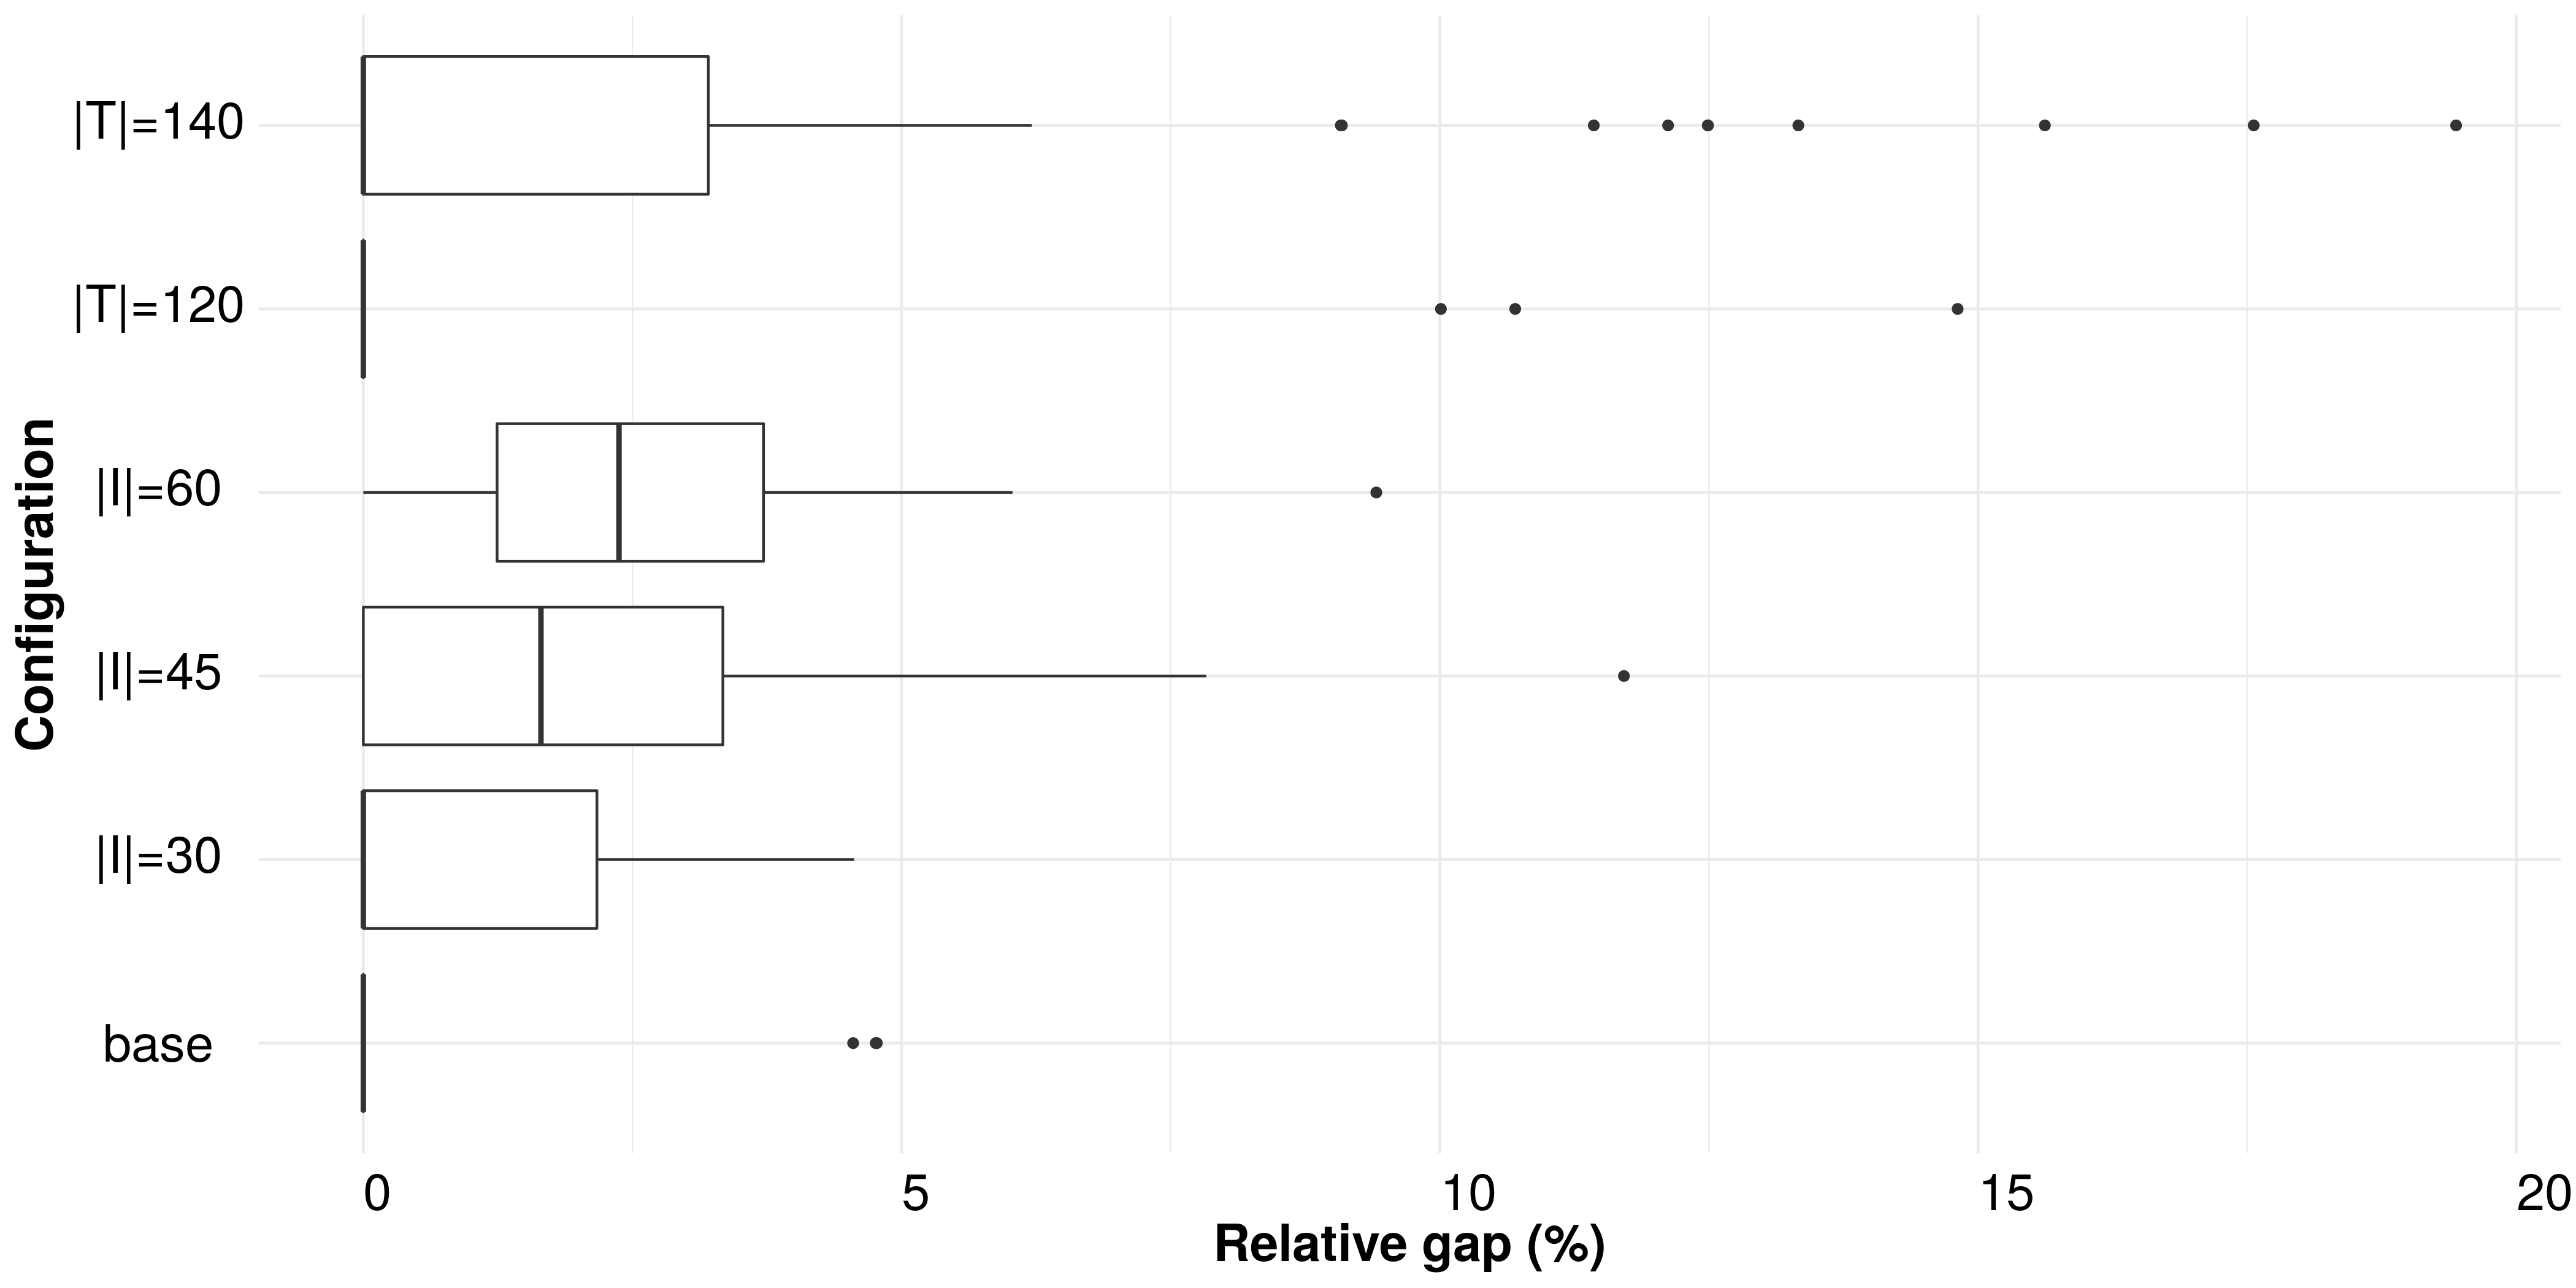
\includegraphics[width=\linewidth]{images/clust1_20190322_gaps.png}
  }
  \only<2>{
    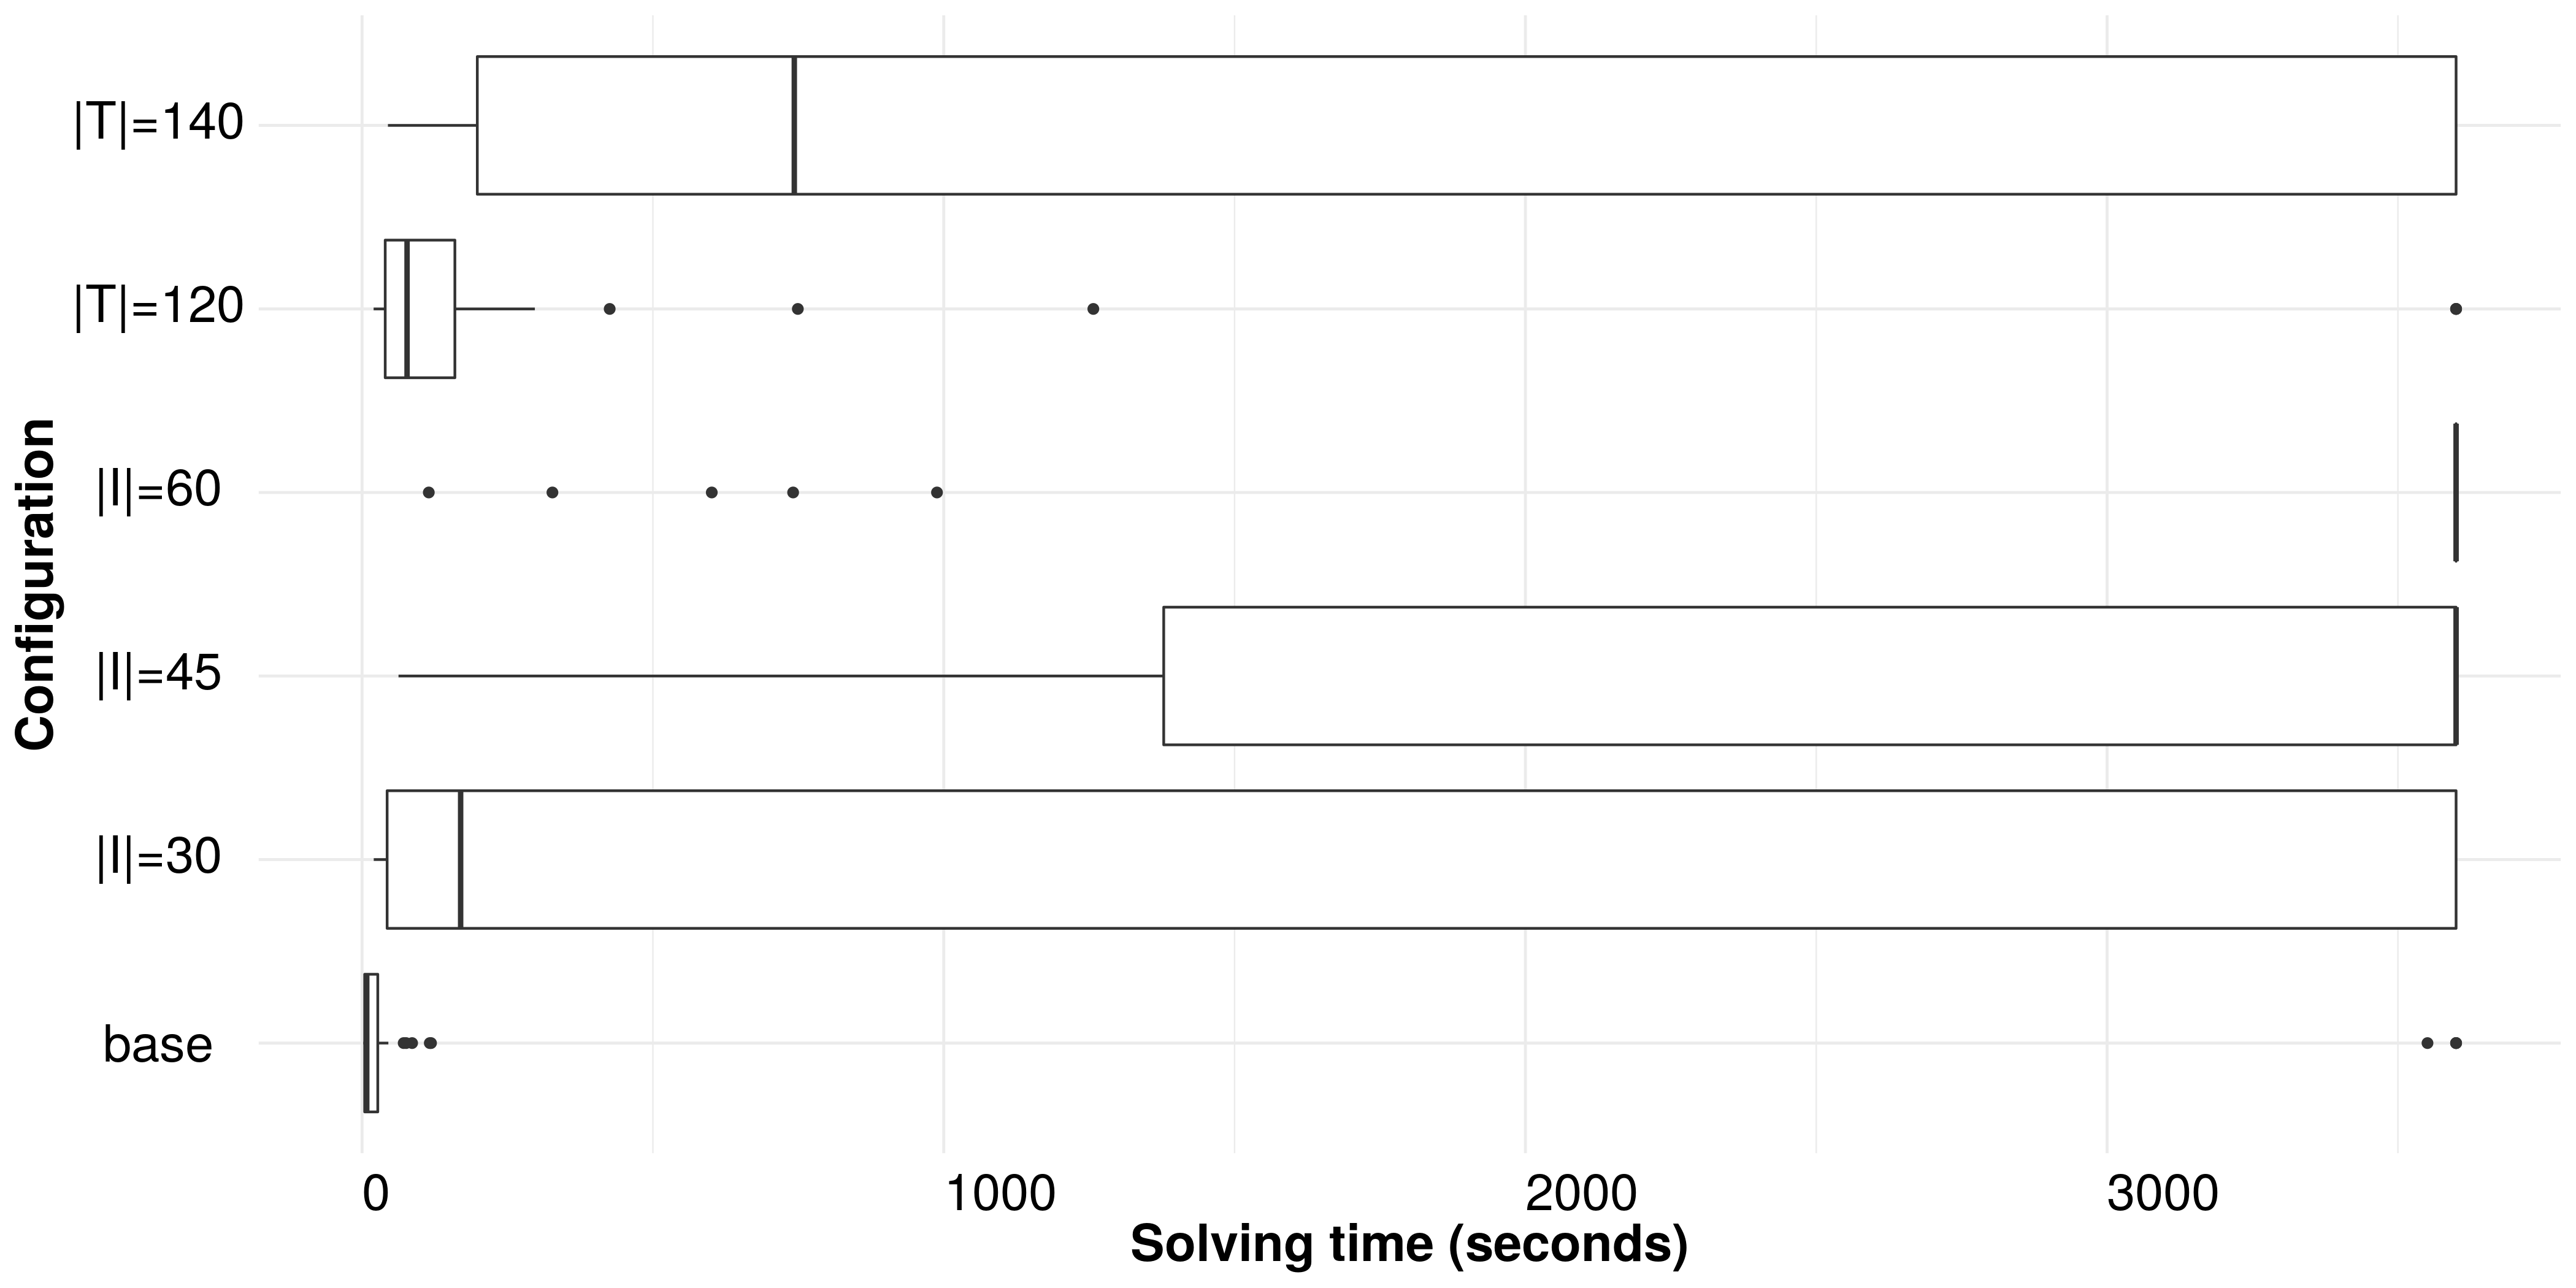
\includegraphics[width=\linewidth]{images/clust1_20190322_times.png}
  }
\end{frame}

\begin{frame}
\frametitle{\textbf{Preliminary conclusions}}
  % \begin{block}{}
    \begin{itemize}[<+->]
    \item \textbf{The long term MFMP problem is presented}
      along with a complexity analysis and a configurable instance generator.
    \item \textbf{Two solving techniques are tested}:
      a MIP model and a Simulated Annealing approach.  
    \item \textbf{Improves are needed} 
      to reduce the model's sensibility to the size of instances.
    \end{itemize}
  % \end{block}  
  % \pause
  % \begin{block}{\textbf{Perspectives}}
  %   \begin{itemize}
  %     \item \textbf{Extend the problem} to include some additional secondary constraints.        
      
        
  %   \end{itemize}
  % \end{block}
  % \pause
  \onslide<+->{
    \textbf{Submission:} Franco Peschiera, Olga Battaïa, Alain Haït, Nicolas Dupin. Long term planning of military aircraft flight and maintenance operations. Annals of Operations Research.
  }
\end{frame}
